% kompilace xelatex prezentace.tex
% dokumentace k beameru: http://ftp.cvut.cz/tex-archive/macros/latex/contrib/beamer/doc/beameruserguide.pdf

% nastavení formátu prezentace 16:9 
\documentclass[czech,aspectratio=169]{beamer}

\usepackage{polyglossia}
\setmainlanguage{czech}

% nastavení vzhledu 
% další možnosti vzhledu viz https://hartwork.org/beamer-theme-matrix/
\usetheme{Madrid}
\usecolortheme{whale}

% vzhled slajdů vnitřní téma (např. vzhled odrážek)
\useinnertheme{rectangles} %možnosti: default circles rectangles rounded inmargin
% vzhled slajdů vnější téma
\useoutertheme{default} %možnosti: default, miniframes, smoothbars, sidebar, split, shadow, tree, smoothtree, infolines

% zavedeme čvutí modou barvu
\definecolor{CVUT}{HTML}{0065BD}
% čvutí modou použijeme jako hlavní barvu prezentace
\setbeamercolor{structure}{bg=white,fg=CVUT}

% jako font prezentace nadefinujeme oficiální ČVUT písmo Technika -- pokud chcete použít, musíte si font nainstalovat nebo jej nahrát na Overleaf
% https://www.cvut.cz/logo-a-graficky-manual  -- inforek, přihlášení přes celoškolské heslo
%\usepackage{fontspec}
%\setsansfont{Technika-Kniha}

% vypneme navigační panel beamer (pro zapnutí zakomentujeme)
\beamertemplatenavigationsymbolsempty

% vygenerujeme slajdy s poznámkami -- ty si můžete vytisknout a mít je na obhajobu s sebou (pokud zapomenete slova, nebo kdyby nefungovalo promítání z nějakého důvodu)
%\setbeameroption{show notes} 

% vygeneruje slajdy s poznámky vhodné pro promítání na dvou monitorech -- na obhajobu nevyužijete
%\usepackage{pgfpages}
%\setbeameroption{show notes on second screen}

% další balíčky
\usepackage{graphicx}
\usepackage{minted}
\usepackage{hyperref}
\usepackage{tikz}
\usetikzlibrary{chains,fit,shapes}

\usepackage{listings} % use code listings package
\lstset{
	basicstyle=\ttfamily,
	columns=fullflexible,
	frame=single,
	breaklines=true
}

% Údaje o prezentaci
\title[Framework for Extraction of Wikipedia Articles Content]{Framework for Extraction of Wikipedia Articles Content}
\subtitle{Diplomová práce}
\institute[FIT ČVUT v Praze]{Fakulta informačních technologií \\ České vysoké učení technické v Praze}
\author[Oleksandr Husiev]{Oleksandr Husiev \\ Vedoucí práce: Ing. Milan Doj{\v c}inovski, Ph. D.}
\date{07. 12. 2021}
\titlegraphic{
\includegraphics[width=.1\textwidth]{logo-cvut}}


\begin{document}
    \begin{frame}
        \titlepage
    \end{frame}
    
    \begin{frame}
        \tableofcontents
    \end{frame}
  
    
    \section{Motivation}
    \begin{frame}{Motivation}
        \begin{itemize}
            \item Knowledge bases are growing up in importance as a Web and enterprise search engine.
            \item Currently knowledge bases cover only specific niches and are
            not useful outside of their primary purpose.
            \item Formatted article data from the Wikipedia in DBPedia is not updated on a regular basis
        \end{itemize}
    \end{frame}

 \section{Thesis goals}

\begin{frame}{Thesis goals}
DBpedia is a crowd-sourced community effort that aims at extraction of information from Wikipedia. 
The main goal of the thesis is to develop a framework for extraction of Wikipedia articles content
, structure and annotations which can be further split into those subgoals:
	
	\begin{itemize}
		\item Accept and process input data in the form of Wikipedia XML dumps
		\item Extract Wikipedia context, page structure, and links.
		\item Provide outputs for context, links and page structure in the form of N-Triples.
		\item Implement language extensibility.
		\item Provide a user interface to interact with the framework.
	\end{itemize}
\end{frame}
    
    \section{Requirements}
    \begin{frame}{Requirements to the Framework}
        \begin{itemize}
            \item Accept input data - support XML dump with up to 20GB of data;
            \item Language extensibility - parse XML in English and at least 4 other languages of choice;
            \item Provide outputs - print all the outputs in the
NIF triples, concatenating processed data from all articles in a single
XML input file and writing the data to .nt output file.
        \end{itemize}
    \end{frame}
    
\begin{frame}{Data Workflow}{General Extraction Framework data workflow}
	\begin{center}
		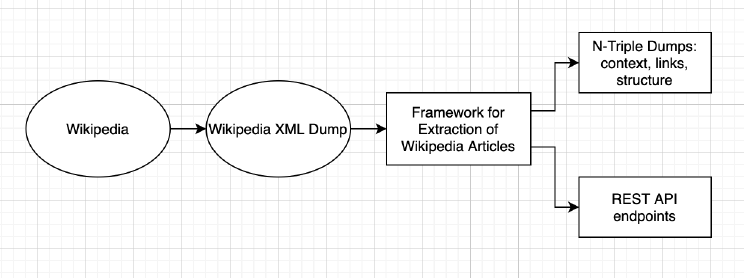
\includegraphics[width=0.6\paperwidth]{data_workflow.png}
	\end{center}
\end{frame}

    \section{Implementation}
	\begin{frame}{Implementation}{ Project Architecture}
		  \begin{itemize}
			\item Interface Layer - used for CLI and REST interface
			\item Logic Layer - used for XML processing of the incoming data
			\item Output Layer - used for tuning parameters for file output.
		\end{itemize}
	\end{frame}

	\begin{frame}{Framework Class Diagram}
		\begin{center}
			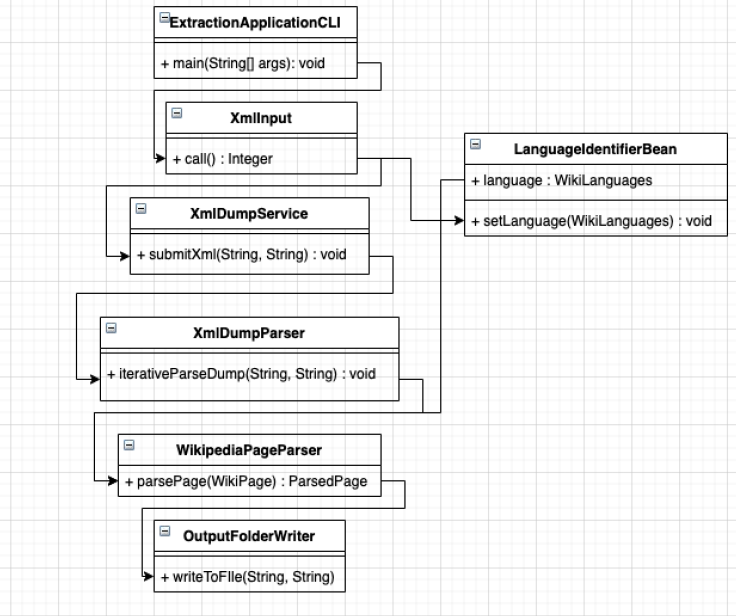
\includegraphics[width=0.55\paperwidth]{framework_diagram.png}
		\end{center}
	\end{frame}

    \section{Tools and Libraries}
    \begin{frame}{Tools and Libraries}
        \begin{itemize}
            \item Java(with Spring Boot and Spring Dependency Injection)
            \item Java Jackson XML Library for XML parsing
            \item picocli for a command-line interface
            \item JUnit for unit testing of the framework
        \end{itemize}
    \end{frame}

	\section{Dynamic Language Support}
	\begin{frame}{Dynamic Language Support}{Support}
		Before the framework starts, it processes the
		configuration file language list.xml that is stored in the configuration folder and instantiates objects during the runtime:
		\begin{center}
			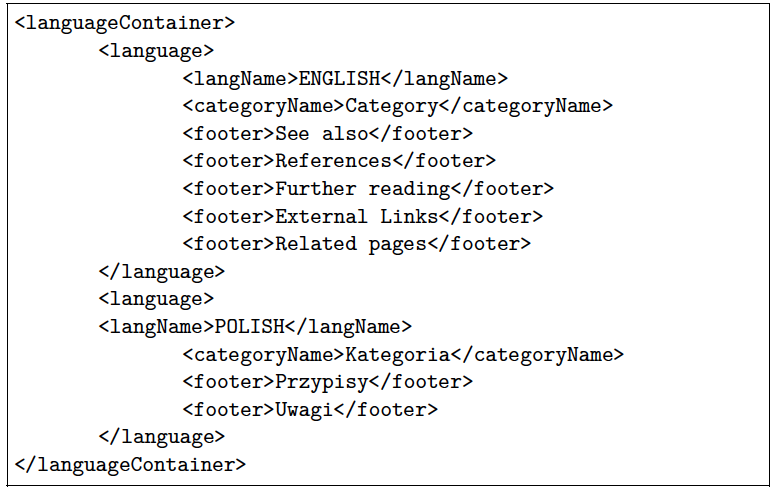
\includegraphics[width=0.45\paperwidth]{lang_config.png}
		\end{center}
	\end{frame}
    
    \section{Testing}
    \begin{frame}{Testing}
    	The framework has been tested during the implementation, using several methodologies
        \begin{itemize}
            \item Unit Testing - to provide test coverage for classes in an isolated environment;
            \item End-to-End Testing: output validation;
            \item End-to-End Testing: scale testing.
        \end{itemize}
    \end{frame}

	\section{End-to-End Testing - Output validation}
	\begin{frame}{Processed Page Structure Output}
		\begin{center}
			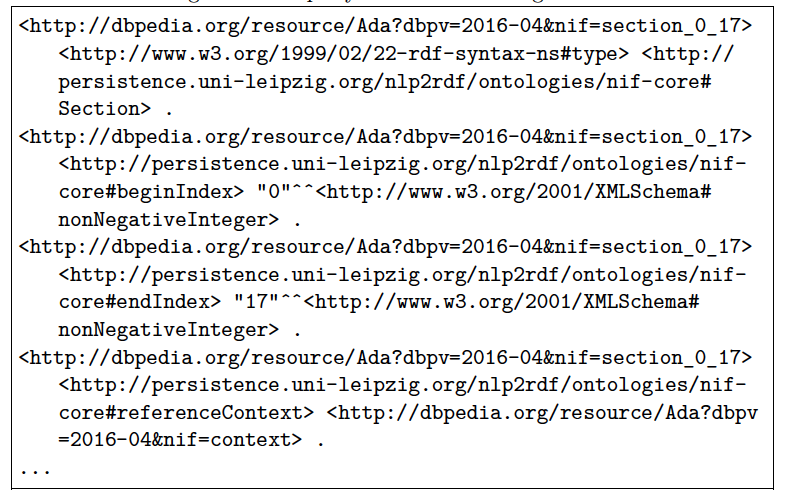
\includegraphics[width=0.65\paperwidth]{nif_page_struct.png}
		\end{center}
	\end{frame}

	\section{End-to-End Testing - Scale Testing}
	\begin{frame}{End-to-End Testing - Scale Testing}
		\begin{itemize}
			\item Total pages parsed: 258. Success rate: 84.88\%. Seconds passed: 31(rate of ~8 articles per second).
			\item Total pages parsed: 2087. Success rate: 88.55\%. Seconds passed: 109(~19 articles per second).
			\item Total pages parsed: 6738. Success rate: 87.90\%. Seconds passed: 237(~28 articles per second).
		\end{itemize}
	
 	\end{frame}

	\section{End-to-End Testing - Language Support}
	\begin{frame}{End-to-End Testing - Language Support}
		After implementing the dynamic language support, I have picked the most popular languages on Wikipedia:
		\begin{itemize}
			\item English: 2,567,509 articles, 22.5\% of the total number of articles;
			\item German: 808,044 articles, 7.1\%;
			\item French: 709,312 articles, 6.2\%;
			\item Polish: 539,688 articles, 4.7\%;
			\item Japanese: 523,629 articles, 4.6\%.
		\end{itemize}
	\end{frame}



    \begin{frame}{Conclusions}
        \begin{itemize}
            \item Accept and process input data in the form of Wikipedia XML
dumps. The Wikipedia XML Dump parsing was achieved. The statistics show that
the parsing success rate averages on 88\% over the large amounts of
articles.
 \item Extract context. Context is extracted and stored in the form of NTriples.
Some of the contexts might still contain traces of the original
XML code.
 \item Extract page structure. Page structure is extracted and recursively
built in the form of N-Triples.
 \item Extract links. Links are extracted, URLs that link them to the page
structure are created.
\item Provide outputs for context, links and page structure in the
form of N-Triples. Output is printed.
\item Implement language extensibility. Language extensibility mechanism
is implemented, new languages can be added in the form of an
XML configuration that is parsed when the application is starting
\item Provide a user interface. User interface is provided in two different
forms
        \end{itemize}
    
    \end{frame}
    
    \begin{frame}{The end}
        \center Thanks for your attention!
        \center Děkuji za pozornost!
    \end{frame}

    \begin{frame}[noframenumbering]{Otázky oponenta}
        Otázka první: Proč?
    
        \vfill
    
        Odpověď: Prostě proto.
    \end{frame}
    
    \begin{frame}[noframenumbering]{Otázky oponenta}
        Otázka druhá: Proč?
    
        \vfill
    
        Odpověď: Prostě proto.
    \end{frame}

\end{document}